\documentclass[
	english,
        solution=true
	]{tudaexercise}

\usepackage[main=english, ngerman]{babel}
\usepackage[babel]{csquotes}

\usepackage{amstext}
\usepackage{amsmath}
\usepackage{amssymb}
\usepackage{graphicx}
\usepackage{setspace}
\usepackage{multicol}
\usepackage{mathtools}
\usepackage{dsfont}
\usepackage{units}
\usepackage{subfigure}
\usepackage{color}
\usepackage{booktabs}
\usepackage{fancyref}
\usepackage{listings}
\usepackage{mathrsfs}
\usepackage{physics}
\usepackage{gauss}
\usepackage{bm}
\usepackage{multirow}
\usepackage{pgfplots}
\usepackage{pgfplotstable}
\usepackage{hyperref}
\usetikzlibrary{patterns}
\usepackage{wasysym}
\usepackage{enumitem}
\usepackage{caption}
\captionsetup{justification=centering}
\usepackage{tcolorbox}



\let\file\texttt
\let\code\texttt
\let\pck\textsf
\let\cls\textsf
\let\tbs\textbackslash


\newlist{checkboxes}{itemize}{1}
\setlist[checkboxes]{label=$\square$, leftmargin=*}


\newtcolorbox{programmingtaskbox}{
  colback=blue!5!white,
  colframe=lightgray!75!black,
  title=Programming Task,
  sharp corners,
  boxrule=0.8pt,
  leftrule=1mm
}


\ConfigureHeadline{
	headline={title}
}

\let\unit\relax

\newcommand{\R}{\mathbb{R}}
\DeclareMathOperator*{\argmax}{arg\,max}
\DeclareMathOperator*{\argmin}{arg\,min}

\begin{document}
\author{Prof. Marcus Rohrbach, Prof. Simone Schaub-Meyer}
\term{Summer Term 2025}
\title[Statistical Machine Learning Exercise 3]{\LARGE Statistical Machine Learning: Exercise 3}
\subtitle{Regression, Kernel Theory, Gaussian Processes, Latent Representation \\ Total Possible Points: 82}
\maketitle

\textcolor{red}{\textbf{Publication Date: June 12th, 21:00 PM}}\\
\textcolor{red}{\textbf{Due Date: July 6th, 23:59 PM}}

\textbf{TEMPLATE:} \href{https://colab.research.google.com/drive/1QM37OJ0yJhGyHJhlzW8UGxJ266q4foF7?usp=sharing}{https://colab.research.google.com/drive/1QM37OJ0yJhGyHJhlzW8UGxJ266q4foF7?usp=sharing}

\begin{task}[points=34]{Regression}
\begin{programmingtaskbox}
Complete the corresponding section of the notebook as part of this task.
\end{programmingtaskbox}
In this exercise, you will implement various kinds of linear regressors using the data \texttt{lin\_reg\_train.txt} and \texttt{lin\_reg\_test.txt}.
The files contain noisy observations from an unknown function $f: \mathbb{R} \mapsto \mathbb{R}$.
In both files, the first column represents the input and the second column represents the output.
You can load the data using \texttt{numpy.loadtxt} and built-in functions for computing the mean.

For all subtasks, assume that the data is identically and independently distributed according to
\begin{equation*}
    y_i = \bm{\Phi}(\mathbf{x_i})^\top \mathbf{w} + \epsilon_i,
\end{equation*}
where
\begin{equation*}
\epsilon_i \sim \mathcal{N}(0, \sigma^2),
\end{equation*}
    and $\Phi: \mathbb{R} \rightarrow \mathbb{R}^n$ is a feature transformation
such that
\begin{equation*}
    \mathbf{y} \sim \mathcal{N}(\bm{\Phi}(\mathbf{X})^\top \mathbf{w}, \sigma^2 \mathbf{I}).
\end{equation*}

Additionally, make sure that your implementations support multivariate inputs. The feature transformations
    are given in each task; if no basis function is stated explicitly, use the data as is, i.e.~$\bm{\Phi}(x) = x$.

\begin{subtask}[points=8, title=Linear Features]
Implement linear ridge regression using linear features, i.e.~the data itself by filling in the ToDos of the corresponding task in the provided Colab Template.
Include an additional input dimension to represent a bias term and use the ridge coefficient $\lambda = 0.01$.
\\
\begin{enumerate}
\item Explain: What is the ridge coefficient and why do we use it? 
\item Derive the optimal model parameters by minimizing the squared error loss function. 
\item Report the root mean squared error of the train and test data under your linear model with linear features. 
\item Include the resulting plot and a short description. 
\end{enumerate}

\begin{solution}

\end{solution}

\end{subtask}

\begin{subtask}[points=8, title=Polynomial Features]
Implement linear ridge regression using a polynomial feature projection by filling in the ToDos of the corresponding task in the provided Colab Template.
Include an additional input dimension to represent a bias term and use the ridge coefficient $\lambda = 0.01$.

For polynomials of degrees 2, 3 and 4:
\begin{enumerate}
\item Report the root mean squared error of the training data and of the testing data under your model with polynomial features.
\item Include the resulting plot and a short description.
\item Why do we call this method \textit{linear} regression despite using polynomials?
\end{enumerate}

\begin{solution}

\end{solution}
\end{subtask}


\begin{subtask}[points=10, title=Bayesian Linear Regression]
Implement Bayesian linear ridge regression by filling in the ToDos of the corresponding task in the provided Colab Template. Assuming that $\mathbf{w}$ follows a multivariate Gaussian distribution, such that
\begin{equation*}
\mathbf{w} \sim \mathcal{N}(\bm{\mu}_0, \bm{\Lambda}_0^{-1}),
\end{equation*}
where ridge regression dictates $\bm{\mu}_0 = \mathbf{0}$ and $\bm{\Lambda}_0 = \lambda \mathbf{I}$.

Here, $\bm{\mu}_0$ is the prior weight mean and $\bm{\Lambda}_0$ is the prior weight precision matrix, i.e.~the inverse of the covariance matrix.
The corresponding posterior parameters can be denoted as $\bm{\mu}_n$ and $\bm{\Lambda}_n$.

Assume $\sigma = 0.1$, use $\lambda = 0.01$, and
include an additional input dimension to represent a bias term.
Use all of the provided training data for a single Bayesian update.

\begin{enumerate}
\item State the posterior distribution of the model parameters $p(\mathbf{w} \mid \mathbf{X}, \mathbf{y})$ (no derivation required). 
\item State the predictive distribution $p(\mathbf{y}_* \mid \mathbf{X}_*, \mathbf{X}, \mathbf{y})$ (no derivation required). 
\item Report the RMSE of the train and test data under your Bayesian model (use the predictive mean). 
\item Report the average log-likelihood of the train and test data under your Bayesian model.
\item Include the resulting plot and a short description. 
\item Explain the differences between linear regression and Bayesian linear regression.
\end{enumerate}

\begin{solution}

\end{solution}
\end{subtask}

 \newpage
\begin{subtask}[points=8, title=Squared Exponential Features]
Implement Bayesian linear ridge regression using squared exponential (SE) features by filling in the ToDos of the corresponding task in the provided Colab Template.
In other words, replace your observed data matrix $\mathbf{X} \in \mathbb{R}^{n \times 1}$ by a feature matrix $\bm{\Phi} \in \mathbb{R}^{n \times k}$,
where
\begin{equation*}
\bm{\Phi}_{ij} = \exp \left( -\frac{1}{2} \beta (\mathbf{X}_i - \alpha_j)^2 \right).
\end{equation*}
Set $k = 20$, $\alpha_j = j * 0.1 - 1$ and $\beta = 10$. Use the ridge coefficient $\lambda = 0.01$ and assume known Gaussian noise with $\sigma = 0.1$.
Include an additional input dimension to represent a bias term.

\begin{enumerate}
\item Report the RMSE of the train and test data under your Bayesian model with SE features. 
\item Report the average log-likelihood of the train and test data under your Bayesian model with SE features. 
\item Include the resulting plot and a short description. 
\item How can SE features be interpreted from a statisticians point of view? What are $\alpha$ and $\beta$ in that context? 
\end{enumerate}

\begin{solution}

\end{solution}
\end{subtask}
\end{task}


\newpage

\begin{task}[points=12]{Gaussian Processes}
\begin{programmingtaskbox}
Complete the corresponding section of the notebook as part of this task.
\end{programmingtaskbox}
\begin{subtask}[title=GP Regression, points= 10]
Implement a Gaussian Process to fit the target function $y = \sin(x) + \cos^2(x)$ with $x \in [0, 0.005, 0.01, 0.015, \ldots, 2\pi]$. First, complete the function \texttt{rbf\_kernel()}.

Use the RBF/Gaussian kernel with a kernel bandwidth of 1, an initial mean of 0 and assume a noise variance of 0.005. Begin with no target data points and, at each iteration, sample a new point from the target function according to the uncertainty of your GP (that is, sample the point where the uncertainty is the highest) and update it. 

Plot your GP (mean and two times the standard deviation) after iterations 1, 2, 5, 10 and 15.
In each figure, plot also the true function as ground truth and add a new marker for each new sampled point. We have provided an example of the plot at iteration 4.

\textbf{Include the plots in your PDF submission.}


\begin{center}
    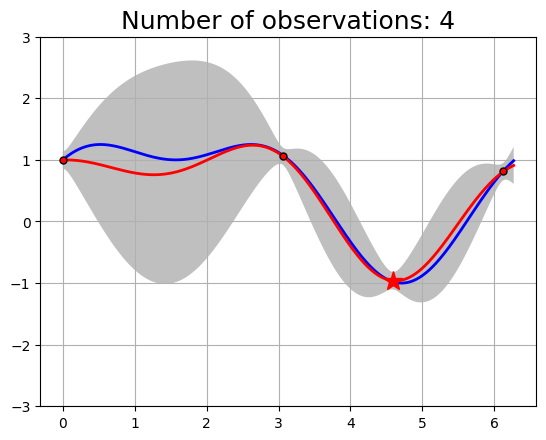
\includegraphics[scale=0.5]{gp_test_example.png}
\end{center}

Notes:
\begin{itemize}
    \item The iteration number is equal to the number of sampled points, e.g. at iteration 5 there are 5 points sampled.
    \item You do not need to strictly follow the given example plot, e.g., using different marker shapes or colors is okay.
    \item The pyplot function \texttt{fill\_between()} might be useful to you.
    \item For the RBF kernel, we use the definition on Slide 47, Lecture 6, where the vertical amplitude is set to 1.
    \item If multiple points have the highest uncertainty, select the one with the lowest index in the dataset.
\end{itemize}
\begin{solution}

\end{solution}
\begin{subtask}[title=Kernel Parameters, points=2]
    Explore various kernel hyperparameters, i.e., \texttt{rbf\_sigma} in the code, and explain how this parameter affects the prediction results.
\end{subtask}

\begin{solution}

\end{solution}
\end{subtask}
\end{task}


\begin{task}[points=28]{Principal Component Analysis}
\begin{programmingtaskbox}
Complete the corresponding section of the notebook as part of this task.
\end{programmingtaskbox}
In this exercise, you will use the dataset \texttt{iris.txt}. It contains data from three kind of Iris flowers (`Setosa', `Versicolour' and `Virginica') with 4 attributes: sepal length, sepal width, petal length, and petal width. Each row contains a sample while the last attribute is the label ($0$ means that the sample comes from a `Setosa' plant, $1$ from a `Versicolour' and $2$ from `Virginica').
(You are allowed to use built-in functions for computing the mean, the covariance, eigenvalues and eigenvectors.)



\begin{subtask}[points=3, title=Data Normalization]
Normalizing the data is a common practice in machine learning. Normalize the provided dataset such that it has zero mean and unit variance per dimension. Why is normalizing important?
Fill in the ToDos of the corresponding task in the provided Colab Template.

\begin{solution}

\end{solution}

\end{subtask}



\begin{subtask}[points=8, title=Principal Component Analysis]
Apply PCA on your normalized dataset and generate a plot showing the proportion (percentage) of the cumulative variance explained (you can use the function \texttt{numpy.cumsum}). 
How many components do you need in order to explain at least $95\%$ of the dataset variance? 
Fill in the ToDos of the corresponding task in the provided Colab Template.
\begin{solution}

\end{solution}
\end{subtask}



\begin{subtask}[points=6, title=Low Dimensional Space]
Using as many components as needed to explain $95\%$ of the dataset variance, generate a scatter plot of the lower-dimensional projection of the data. Use different colors or symbols for data points from different classes. Fill in the ToDos of the corresponding task in the provided Colab Template. What do you observe? 


\begin{solution}

\end{solution}

\end{subtask}



\begin{subtask}[points=6, title=Projection to the Original Space]
Reconstruct the original dataset by using different number of principal components. Using the normalized root mean square error (NRMSE) as a metric, fill the table below (error per input versus the amount of principal components used). Fill in the ToDos of the corresponding task in the provided Colab Template.

\begin{tabular}{c|r|r|r|r}
N. of components & $x_1$ & $x_2$ & $x_3$ & $x_4$ \\
\hline
1 & & & & \\
2 & & & & \\
3 & & & & \\
4 & & & &
\end{tabular}

Remember that in the first step you normalized the data.

\begin{solution}

\end{solution}
\end{subtask}

\newpage

\begin{subtask}[points=5, title=Kernel PCA]
Throughout this class we have seen that PCA is an easy and efficient way to reduce the dimensionality of some data. However, it is able to detect only linear dependences among data points. A more sophisticated extension to PCA, \emph{Kernel PCA}, is able to overcome this limitation. 
This question asks you to deepen this topic by conducting some research by yourself: explain what Kernel PCA is, how it works and what are its main limitations. Be as concise (but clear) as possible.

\begin{solution}

\end{solution}
\end{subtask}
\end{task}


\begin{task}[points=8]{Kernel Construction}
Let \( X \) be a non-empty set. A \textbf{kernel} is a symmetric function \( k : X \times X \rightarrow \mathbb{R} \). The set \( X \) can have arbitrary structure (e.g., real vector space, graphs, images, strings, etc.). 

A kernel \( k \) is called \textbf{positive definite} if for all finite subsets \( \{x_i\}_{i=1}^n \subseteq X \), the corresponding kernel matrix \( K \in \mathbb{R}^{n \times n} \) with entries \( K_{ij} = k(x_i, x_j) \) is positive semi-definite (check Lecture 6 slide 9), i.e.,

\[
\forall \alpha \in \mathbb{R}^n,\quad \alpha^\top K \alpha \geq 0.
\]

Let \( k_1, k_2 : X \times X \rightarrow \mathbb{R} \) be two positive definite kernels. We are to prove that the following operations yield valid positive definite kernels:

\begin{enumerate}
    \item \( k(x, x') = k_1(x, x') + k_2(x, x') \) 
    \item \( k(x, x') = c \cdot k_1(x, x') \), for \( c \geq 0 \) 
    \item \( k(x, x') = k_1(x, x') \cdot k_2(x, x') \) 
    \item \( k(x, x') = k_1(f(x), f(x')) \) for some function \( f : X \rightarrow X \) 
\end{enumerate}


\begin{solution}

\end{solution}


\end{task}
\end{document}